\documentclass{beamer}

\usepackage{beamerouterthemeandrena}
\usepackage[utf8]{inputenc}
\usepackage{babel}
\usepackage{graphicx}
\usepackage{tikz}

\title{Hello Cargo}

\begin{document}



\begin{frame}
    \begin{tikzpicture}[remember picture,overlay]
        \node[inner sep=0] at (current page.center) {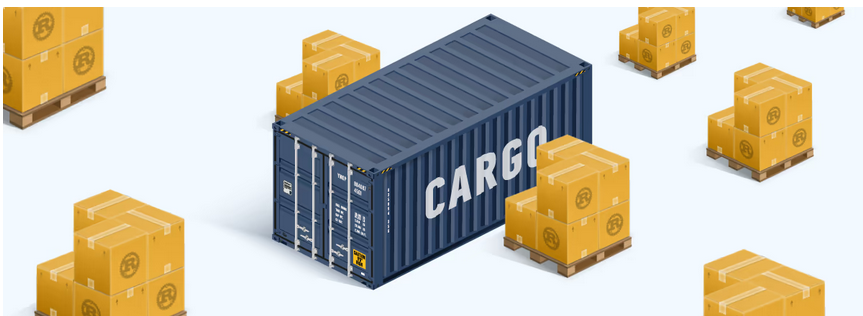
\includegraphics[width=\paperwidth,height=\paperheight]{images/cargo-title-image}};
    \end{tikzpicture}

\end{frame}


\begin{frame}
		\frametitle{What is Cargo?}
		\begin{itemize}
			\item Cargo is Rust's build system and package manager
            \vspace{\baselineskip}
			\item Bundled with Rust installation (cargo -{}-version)
            \vspace{\baselineskip}
			\item Source files should live in \textit{src} directory
            \vspace{\baselineskip}
			\item \href{https://crates.io}{crates.io} is central package registry
		\end{itemize}
\end{frame}

\begin{frame}
	\frametitle{What is Cargo?}
    \begin{figure}
        \centering
        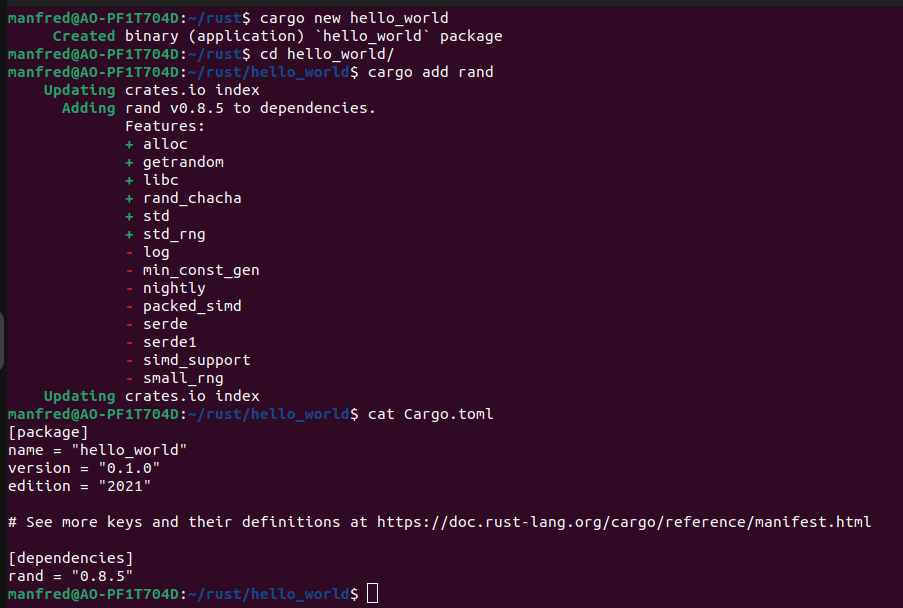
\includegraphics[width=0.9\linewidth]{images/cargo-toml}
    \end{figure}
\end{frame}

\begin{frame}
    \frametitle{Building with Cargo}
   	\begin{itemize}
        \item To build a project use \textit{cargo build} and \textit{./target/debug/hello\_cargo} to run executable
        \vspace{\baselineskip}
        \item \textit{cargo run} can be used to build and run in one step
        \vspace{\baselineskip}
        \item For finished project use \textit{cargo build -{}-release}
    \end{itemize}
\end{frame}

\begin{frame}
    \frametitle{Rust editions}
    \begin{itemize}
        \item Rust language has six-week release cycle -- smaller updates more frequently
        \item Every two or three years a new Rust edition is produced
        \item New editions ship as part of the six-week release process
        \item Editions serve different purposes for different people
        \item The edition key in Cargo.toml indicates which edition the compiler should use for code.
        \item All Rust compiler version support any edition that existed prior to that compilers release
    \end{itemize}
\end{frame}



\begin{frame}
\begin{tikzpicture}[remember picture,overlay]
    \node[inner sep=0] at (current page.center) {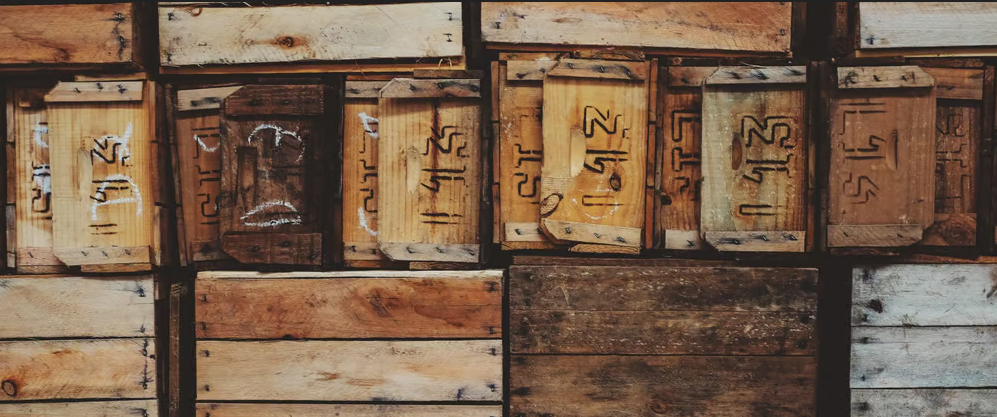
\includegraphics[width=\paperwidth,height=\paperheight]{images/module-system-title-image}};
    \node[text=white,font=\LARGE] at (current page.center) {Module system -- Crates and Modules};
\end{tikzpicture}

\end{frame}



\begin{frame}
    \frametitle{How to organize code}
    \begin{itemize}
        \item Crate: Tree of modules producing a library or executable.
        \item Crate Root is source file that Rust compiler starts from to make up root module of crate
        \begin{itemize}
            \item[$\diamond$] Binary Crates – Crate Root: src/main.rs
            \item[$\diamond$] Library Crates – Crate Root: src/lib.rs
        \end{itemize}
        \vspace{\baselineskip}
        \item Package: A bundle of one or more crates
        \vspace{\baselineskip}
        \item Module: Collection of items like functions, structs, traits and impl blocks                \begin{itemize}
            \item[$\diamond$] The use keyword creates shortcuts to items
        \end{itemize}
        \vspace{\baselineskip}
        \item Paths: A way of naming an item to show Rust where to find an item in a module tree
        \begin{itemize}
            \item[$\diamond$] Absolute path – Full path starting from create root
            \item[$\diamond$] Relative Path – Starts from current module (self, super)
        \end{itemize}
    \end{itemize}
\end{frame}


\begin{frame}
    \frametitle{How to organize code}
    When declaring a module in crate root, the compiler looks in these places
    \begin{itemize}
        \item Inline
        \item In src/$<$module-name$>$.rs
        \item In src/$<$module-name$>$/mod.rs
     \end{itemize}
\end{frame}

\begin{frame}
    \frametitle{How to organize code}
\begin{figure}
    \centering
    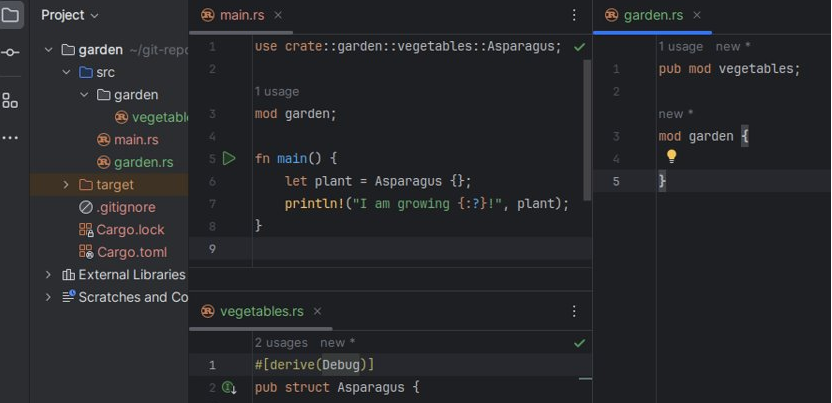
\includegraphics[width=0.9\linewidth]{images/modules-example}
\end{figure}
\end{frame}

\begin{frame}
    \frametitle{References}
    \begin{enumerate}
        \item \href{https://media.dev.to/cdn-cgi/image/width=1000,height=420,fit=cover,gravity=auto,format=auto/https\%3A\%2F\%2Fdev-to-uploads.s3.amazonaws.com\%2Fi\%2Fvd28y0mx3grcgrfduwkd.jpg}{\textit{module-system-title-image}}
        \item \href{https://jfrog.com/devops-tools/article/how-to-run-a-private-cargo-registry/}{\textit{cargo-title-image}}
    \end{enumerate}
\end{frame}


\end{document}
